\section{Introduction}
\label{sec:precise-alignment-intro}

The previous chapter established a LiDAR-inertial SLAM pipeline capable of performing without continuous GNSS availability, providing robust trajectory estimation and semi-dense environmental mapping across vineyard rows. While this system delivers the localisation accuracy required for autonomous navigation between vines, it does not, by itself, provide the centimetre-scale spatial accuracy necessary for robotic pruning. When a manipulator arm must reach a specific cane at a specific cut-point, the acceptable localisation error is smaller than what global SLAM can guarantee. This chapter aims to address that gap through a second-stage localisation refinement step that aligns the robot's perception of its environment with a pre-built high-fidelity vine model.

Whereas the SLAM system presented in \cref{chap:SLAM} is designed to operate across the full annual growth cycle of the vine, the precise-alignment stage described here is explicitly scoped to the winter pruning season. Robotic pruning is inherently a winter task: grapevines are pruned during dormancy, when they have shed their foliage and only the bare woody cane and trunk structure remains. The point cloud registration pipeline presented in this chapter exploits that leafless condition, as bare-wood geometry provides clean, unoccluded structure for alignment. All experiments and pipeline design decisions therefore assume dormant-season vine structure; vines carrying a full canopy are outside the scope of this work.

\subsection{System Context}
\label{subsec:system-context}

Central to the pruning localisation workflow described in this thesis is a 3D Gaussian Splatting (3DGS) model of each vine, constructed offline from imagery collected during a prior scanning pass. The reconstruction pipeline applies Structure from Motion (SfM) photogrammetry to these images, recovering a dense 3D point cloud and camera trajectory via bundle adjustment. The resulting point cloud forms the geometric backbone of the 3DGS model and is registered within a global Local East-North-Up (ENU) reference frame. Because SfM jointly optimises camera poses and 3D structure through reprojection minimisation, the reconstructed geometry is internally consistent and, once georeferenced, constitutes a reliable proxy for the true physical vine geometry. All downstream tasks — cut-point detection, path planning for the robotic arm, and collision avoidance — are computed against this 3DGS model in simulation. For these simulated operations to correspond faithfully to the real world, the robot's pose relative to the simulated vine (i.e.\ the 3DGS reconstruction) must match its true pose relative to the physical vine.

When the robot arrives at a target vine during an autonomous pruning mission, its pose is known only to the accuracy of the SLAM system described in \cref{chap:SLAM}. This accuracy is sufficient for navigation but insufficient for manipulation. The precise-alignment stage presented here corrects the residual misalignment by registering a real-time point cloud of the physical vine, acquired at the site, against the SfM point cloud extracted from the 3DGS model. The resulting rigid-body transformation is used to update the robot's estimated pose, thereby aligning the simulated and physical scenes before any pruning motion is executed. The overall system context is illustrated in \cref{fig:pa-system-context}.

\begin{figure}[htbp]
  \centering
  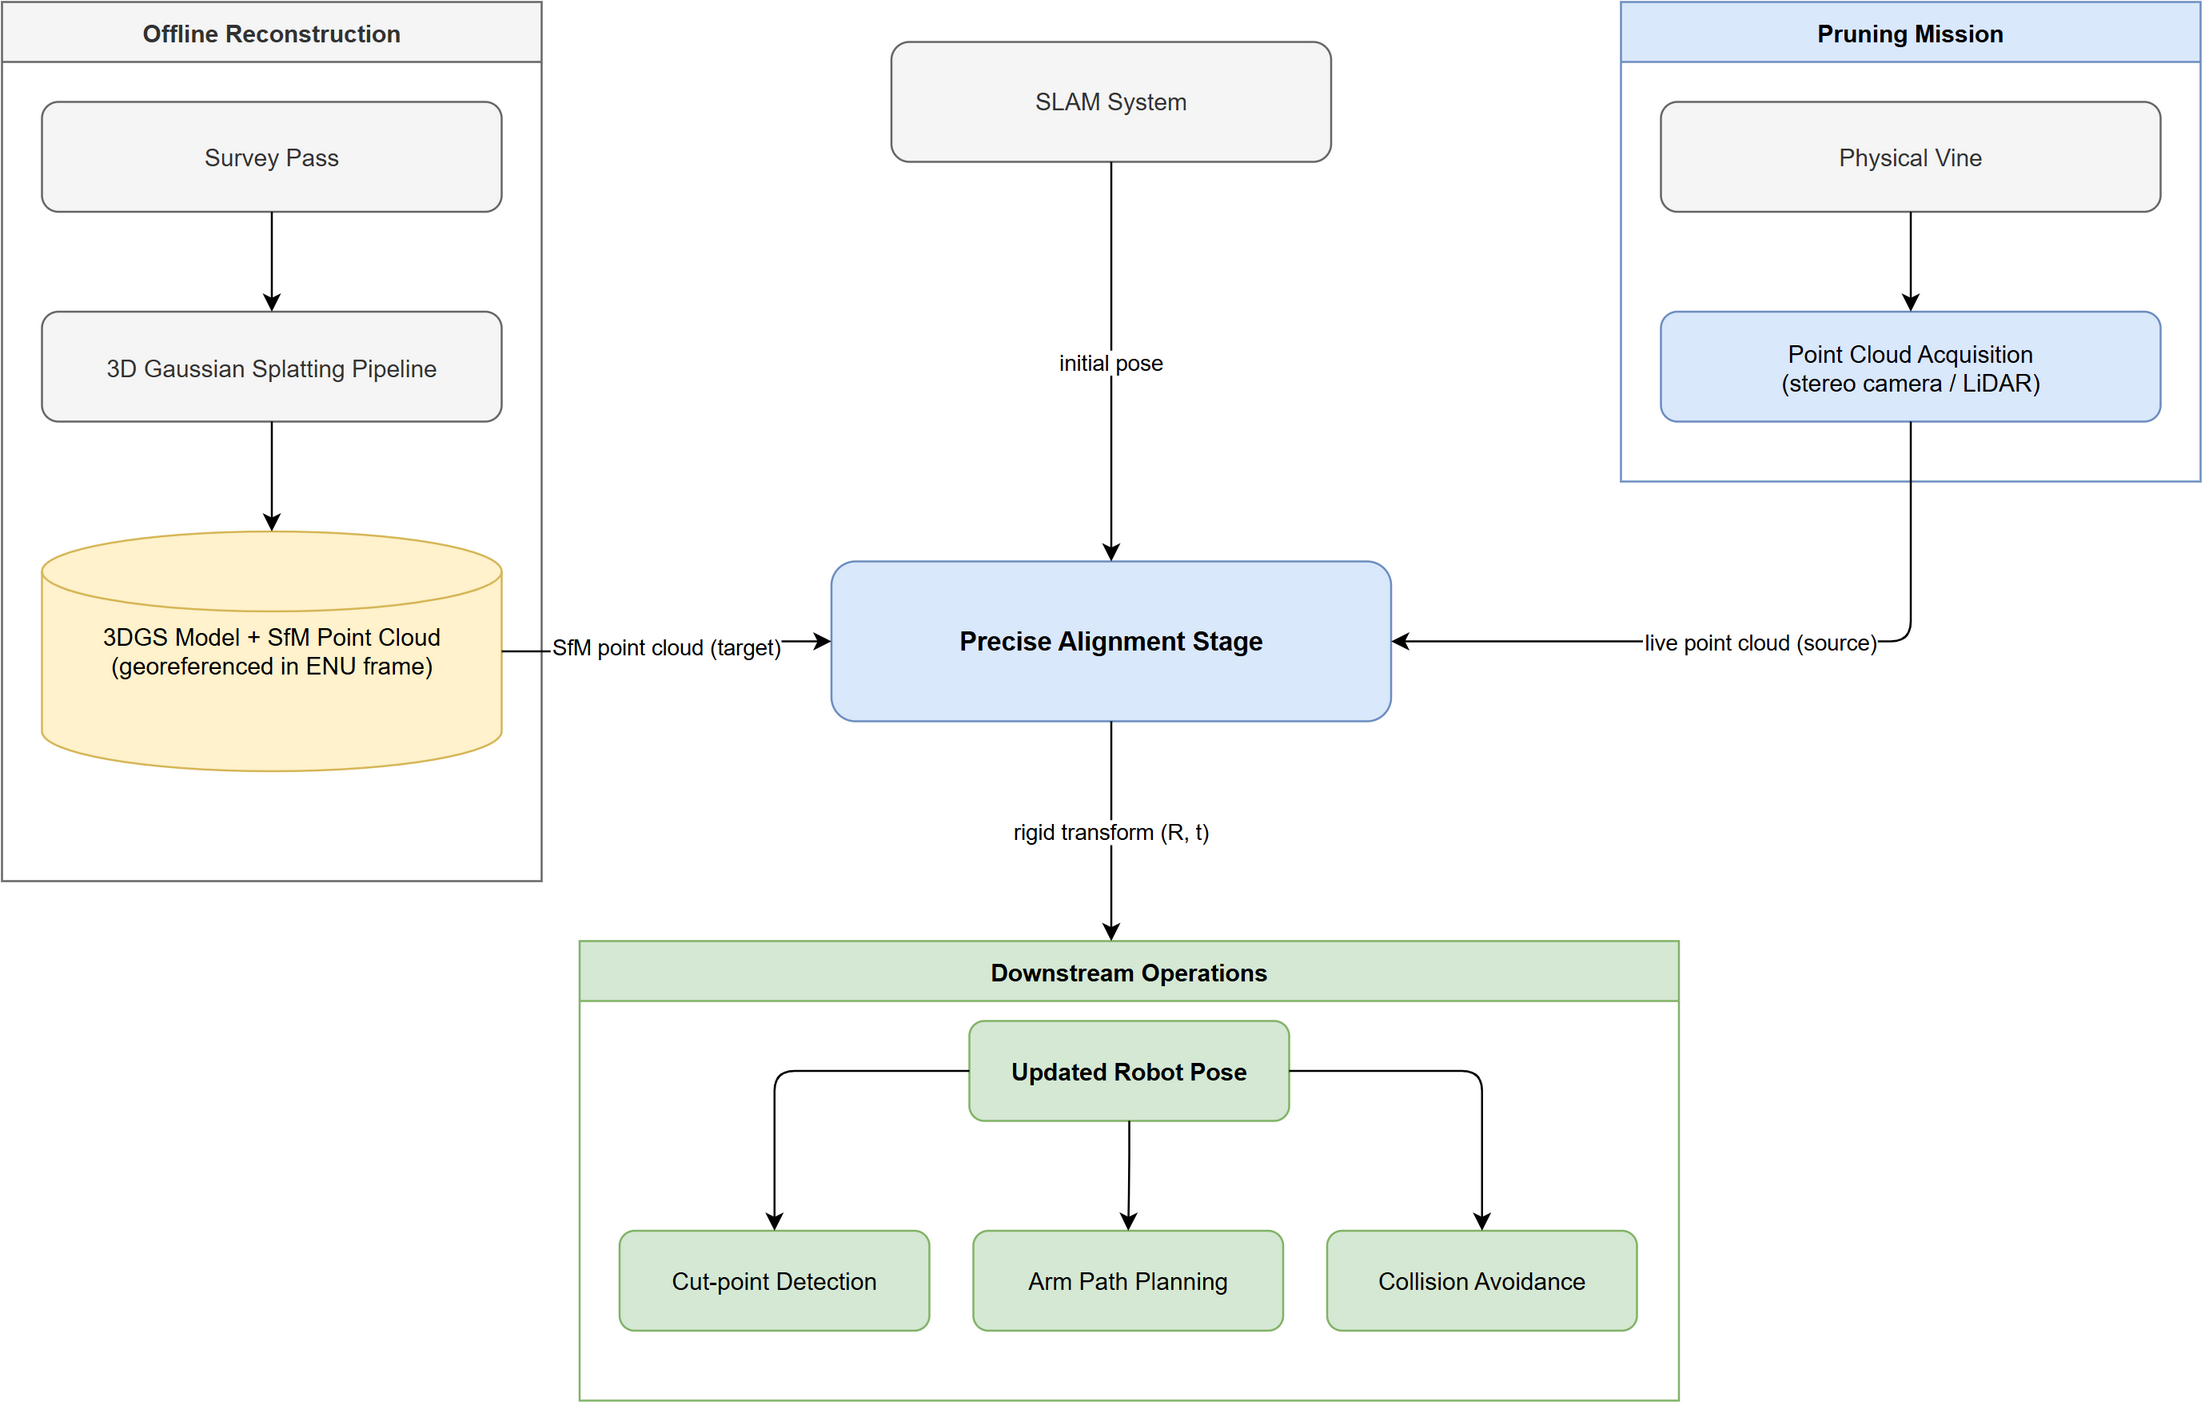
\includegraphics[width=\linewidth]{4-precise-alignment/4-intro/figures/pa-system-context}
  \caption{System context for the precise-alignment stage. Offline 3DGS
           reconstruction and a SLAM-derived initial pose are combined with a
           live sensor point cloud to produce a refined pose for downstream
           manipulation.}
  \label{fig:pa-system-context}
\end{figure}

\subsection{Approach Overview}
\label{subsec:approach-overview}

The precise-alignment pipeline proceeds through the following stages, as illustrated schematically in \cref{fig:pa-approach-overview}:

\begin{enumerate}
    \item The robot halts in front of the target vine and acquires a dense point cloud of the vine structure. Two sensing modalities are evaluated in this chapter: depth point clouds generated from a stereo camera, and dense maps built from a hybrid solid-state LiDAR sensor (Livox Mid-360).
    \item The acquired point cloud is passed through a modality-specific preprocessing pipeline that isolates the vine's structural geometry by removing noise and non-structural clutter, and downsamples the pointcloud to a resolution suitable for registration.
    \item The preprocessed source cloud is registered against the target cloud derived from the SfM reconstruction of the 3DGS model using the Generalised Iterative Closest Point (GICP) algorithm \cite{segalGeneralizedICP2009}.
    \item The recovered transformation is applied to update the robot's internal localisation, correcting its estimated pose relative to the vine. This updated pose is consumed by the arm path planner, ensuring that simulated cut-points correspond to their physical counterparts.
\end{enumerate}

\begin{figure}[htbp]
  \centering
  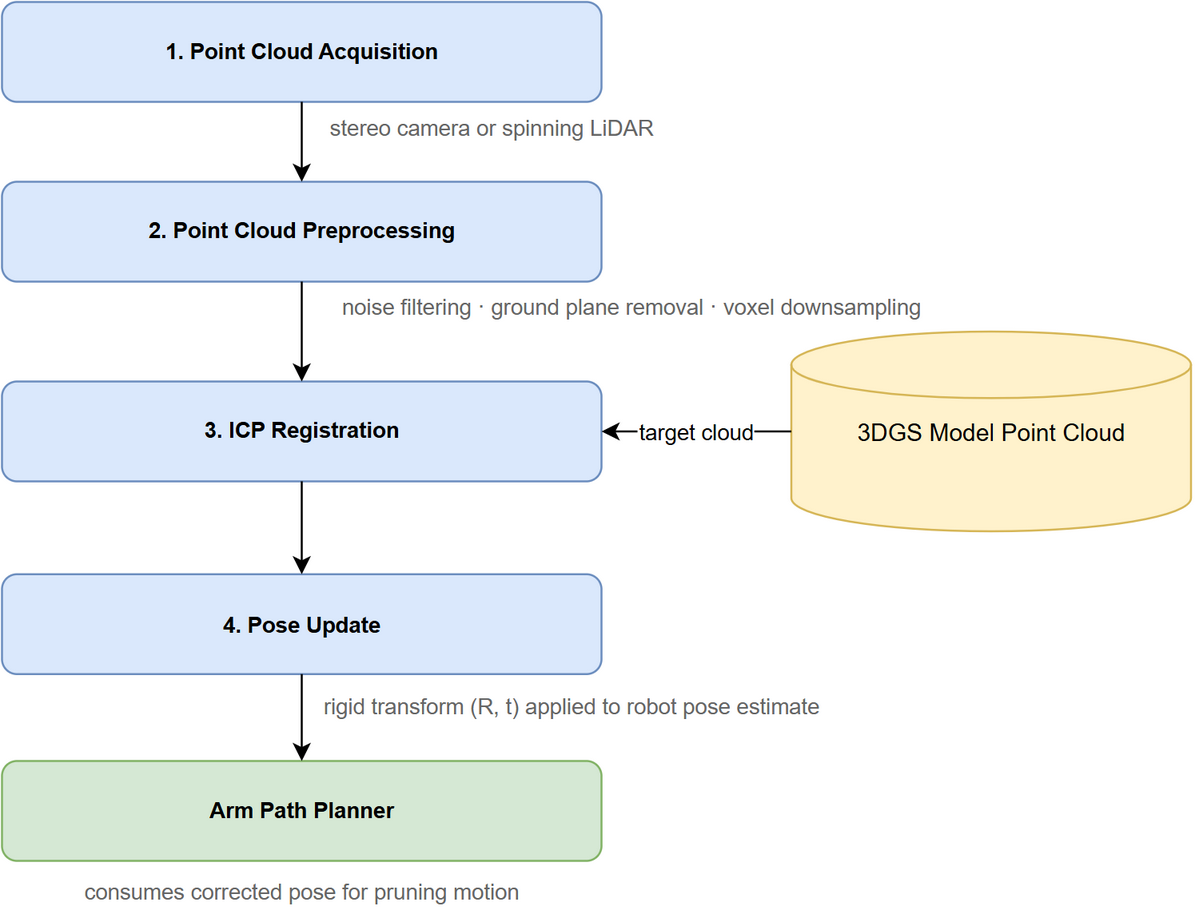
\includegraphics[width=0.65\linewidth]{4-precise-alignment/4-intro/figures/pa-approach-overview}
  \caption{Overview of the four-stage precise-alignment pipeline}
  \label{fig:pa-approach-overview}
\end{figure}

Each stage of this pipeline draws on a distinct body of prior work. This chapter is structured as follows. \Cref{sec:precise-alignment-related-work} reviews prior work on point cloud registration for agricultural and robotic applications, with particular attention to ICP variants and vine-specific sensing modalities. \Cref{sec:precise-alignment-methodology} details the full data processing and registration pipeline, including sensor configuration, preprocessing steps, and ICP parameterisation. \Cref{sec:precise-alignment-results} presents quantitative and qualitative results for both sensing modalities across a set of vineyard test cases. \Cref{sec:precise-alignment-discussion} discusses the relative merits and failure modes of each approach, and \cref{sec:precise-alignment-summary} summarises the key findings.